\subsection{RQ2: Retries}
\begin{figure} 
  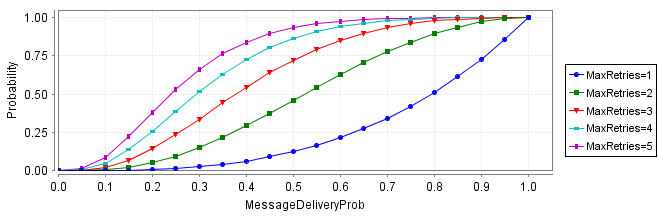
\includegraphics[width=\textwidth]{RQ2-small.png}
  \caption{Probability of Property Satisfied vs Message Success Probability}
  \label{RQ2-small}
\end{figure}

In this experiment we repeat experiment 1 by varying the number of retries from 1 to 5. The results are shown in Figure \ref{RQ2-small}. We can see that even a small number of retries can quickly improve the reliability of the system. For example: with 50\% probability of message delivery, retrying 5 times already gives us a system reliability of over 90\%. It is worth noting that the systems we have modeled don't updates their status periodically. Therefore the chances to update are limited. In a system where sensors have periodic updates, the system should be even more reliable because redundant information would be flowing in the system by design.

\subsection{RQ2: Retries}
\begin{figure} 
  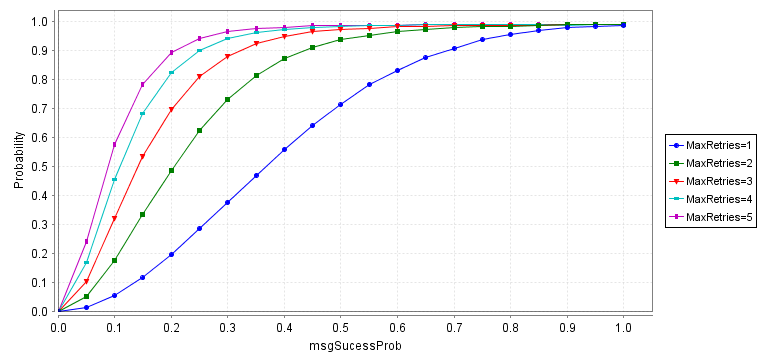
\includegraphics[width=\textwidth]{RQ2-large.png}
  \caption{Probability of Property Satisfied vs Message Success Probability}
  \label{RQ2-large}
\end{figure}

Figure \ref{RQ2-large} shows the result for the large model. This experiment took approximately 1.5 hours to collect readings from all points. Once again we see a dramatic improvement in the reliability of the system when a small bounded number of retries are allowed. Comparing the two models we observe that the larger model shows improvement of system success probability much quicker than the smaller model. This is because of the inherent redundancy in the system.